\documentclass[]{article}
\usepackage{lmodern}
\usepackage{amssymb,amsmath}
\usepackage{ifxetex,ifluatex}
\usepackage{fixltx2e} % provides \textsubscript
\ifnum 0\ifxetex 1\fi\ifluatex 1\fi=0 % if pdftex
  \usepackage[T1]{fontenc}
  \usepackage[utf8]{inputenc}
\else % if luatex or xelatex
  \ifxetex
    \usepackage{mathspec}
  \else
    \usepackage{fontspec}
  \fi
  \defaultfontfeatures{Ligatures=TeX,Scale=MatchLowercase}
\fi
% use upquote if available, for straight quotes in verbatim environments
\IfFileExists{upquote.sty}{\usepackage{upquote}}{}
% use microtype if available
\IfFileExists{microtype.sty}{%
\usepackage{microtype}
\UseMicrotypeSet[protrusion]{basicmath} % disable protrusion for tt fonts
}{}


\usepackage{longtable,booktabs}
\usepackage{graphicx}
% grffile has become a legacy package: https://ctan.org/pkg/grffile
\IfFileExists{grffile.sty}{%
\usepackage{grffile}
}{}
\makeatletter
\def\maxwidth{\ifdim\Gin@nat@width>\linewidth\linewidth\else\Gin@nat@width\fi}
\def\maxheight{\ifdim\Gin@nat@height>\textheight\textheight\else\Gin@nat@height\fi}
\makeatother
% Scale images if necessary, so that they will not overflow the page
% margins by default, and it is still possible to overwrite the defaults
% using explicit options in \includegraphics[width, height, ...]{}
\setkeys{Gin}{width=\maxwidth,height=\maxheight,keepaspectratio}
\IfFileExists{parskip.sty}{%
\usepackage{parskip}
}{% else
\setlength{\parindent}{0pt}
\setlength{\parskip}{6pt plus 2pt minus 1pt}
}
\setlength{\emergencystretch}{3em}  % prevent overfull lines
\providecommand{\tightlist}{%
  \setlength{\itemsep}{0pt}\setlength{\parskip}{0pt}}
\setcounter{secnumdepth}{5}

%%% Use protect on footnotes to avoid problems with footnotes in titles
\let\rmarkdownfootnote\footnote%
\def\footnote{\protect\rmarkdownfootnote}

%%% Change title format to be more compact
\usepackage{titling}

% Create subtitle command for use in maketitle
\providecommand{\subtitle}[1]{
  \posttitle{
    \begin{center}\large#1\end{center}
    }
}

\setlength{\droptitle}{-2em}

\RequirePackage[]{D:/R-4.4.1/library/BiocStyle/resources/tex/Bioconductor}

\bioctitle[]{How to Use \texttt{ANPELA}?}
    \pretitle{\vspace{\droptitle}\centering\huge}
  \posttitle{\par}
\author[1]{Huaicheng Sun}
\author[1]{Yuan Zhou}
\author[1]{Yuxuan Liu}
\author[1]{Feng Zhu\thanks{\ttfamily zhufeng@zju.edu.cn}}
\affil[1]{College of Pharmaceutical Sciences, Zhejiang University, China<br><br><span style="font-style:italic;">For technical issues, please contact Huaicheng Sun at <a href="mailto:sunhc@zju.edu.cn">sunhc@zju.edu.cn</a>.</span>}
    \preauthor{\centering\large\emph}
  \postauthor{\par}
      \predate{\centering\large\emph}
  \postdate{\par}
    \date{04 December, 2024}


% code highlighting

\newcommand{\hlnum}[1]{\textcolor[rgb]{0.816,0.125,0.439}{#1}}%
\newcommand{\hlstr}[1]{\textcolor[rgb]{0.251,0.627,0.251}{#1}}%
\newcommand{\hlcom}[1]{\textcolor[rgb]{0.502,0.502,0.502}{\textit{#1}}}%
\newcommand{\hlopt}[1]{\textcolor[rgb]{0,0,0}{#1}}%
\newcommand{\hlstd}[1]{\textcolor[rgb]{0.251,0.251,0.251}{#1}}%
\newcommand{\hlkwa}[1]{\textcolor[rgb]{0.125,0.125,0.941}{#1}}%
\newcommand{\hlkwb}[1]{\textcolor[rgb]{0,0,0}{#1}}%
\newcommand{\hlkwc}[1]{\textcolor[rgb]{0.251,0.251,0.251}{#1}}%
\newcommand{\hlkwd}[1]{\textcolor[rgb]{0.878,0.439,0.125}{#1}}%
\let\hlipl\hlkwb
%
\usepackage{fancyvrb}
\newcommand{\VerbBar}{|}
\newcommand{\VERB}{\Verb[commandchars=\\\{\}]}
\DefineVerbatimEnvironment{Highlighting}{Verbatim}{commandchars=\\\{\}}
%
\newenvironment{Shaded}{\begin{myshaded}}{\end{myshaded}}
% set background for result chunks
\let\oldverbatim\verbatim
\renewenvironment{verbatim}{\color{codecolor}\begin{myshaded}\begin{oldverbatim}}{\end{oldverbatim}\end{myshaded}}
%
\newcommand{\KeywordTok}[1]{\hlkwd{#1}}
\newcommand{\DataTypeTok}[1]{\hlkwc{#1}}
\newcommand{\DecValTok}[1]{\hlnum{#1}}
\newcommand{\BaseNTok}[1]{\hlnum{#1}}
\newcommand{\FloatTok}[1]{\hlnum{#1}}
\newcommand{\ConstantTok}[1]{\hlnum{#1}}
\newcommand{\CharTok}[1]{\hlsng{#1}}
\newcommand{\SpecialCharTok}[1]{\hlsng{#1}}
\newcommand{\StringTok}[1]{\hlsng{#1}}
\newcommand{\VerbatimStringTok}[1]{\hlsng{#1}}
\newcommand{\SpecialStringTok}[1]{\hlsng{#1}}
\newcommand{\ImportTok}[1]{{#1}}
\newcommand{\CommentTok}[1]{\hlcom{#1}}
\newcommand{\DocumentationTok}[1]{\hlcom{#1}}
\newcommand{\AnnotationTok}[1]{\hlcom{#1}}
\newcommand{\CommentVarTok}[1]{\hlcom{#1}}
\newcommand{\OtherTok}[1]{{#1}}
\newcommand{\FunctionTok}[1]{\hldef{#1}}
\newcommand{\VariableTok}[1]{\hldef{#1}}
\newcommand{\ControlFlowTok}[1]{\hlkwd{#1}}
\newcommand{\OperatorTok}[1]{\hlopt{#1}}
\newcommand{\BuiltInTok}[1]{{#1}}
\newcommand{\ExtensionTok}[1]{{#1}}
\newcommand{\PreprocessorTok}[1]{\textit{#1}}
\newcommand{\AttributeTok}[1]{{#1}}
\newcommand{\RegionMarkerTok}[1]{{#1}}
\newcommand{\InformationTok}[1]{\textcolor{messagecolor}{#1}}
\newcommand{\WarningTok}[1]{\textcolor{warningcolor}{#1}}
\newcommand{\AlertTok}[1]{\textcolor{errorcolor}{#1}}
\newcommand{\ErrorTok}[1]{\textcolor{errorcolor}{#1}}
\newcommand{\NormalTok}[1]{\hldef{#1}}
%
\AtBeginDocument{\bibliographystyle{D:/R-4.4.1/library/BiocStyle/resources/tex/unsrturl}}


\begin{document}
\maketitle
\begin{abstract}
Single-cell proteomics (SCP) has emerged as a powerful technique that significantly advances our understanding of complex biological systems with new level of granularity. Because of the extreme difficulty in processing SCP data, ANPELA was developed for identifying the optimal workflow based on a well-designed assessment strategy. \textbf{ANPELA} is a \textbf{user-centric} and \textbf{application-oriented} tool which is capable of navigating the data processing for SCP. \textbf{ANPELA 3.0} has significantly improved its practicality, focusing primarily on the following points: \textbf{1}. multi-scenarios deployment (versatile choices meet diverse user needs); \textbf{2}. data security (local execution ensures data confidentiality); \textbf{3}. open source (modular codes facilitate readers' free editing); and \textbf{4}. user-friendly interface (the visual interface enhances user application). The local software and webserver of ANPELA are available at http://idrblab.org/anpela2024.
\end{abstract}

\packageVersion{ANPELA 1.0.0}

{
\setcounter{tocdepth}{2}
\tableofcontents
\newpage
}
\section{Introduction}\label{introduction}

\texttt{ANPELA} includes various built-in processing methods for Cytometry Single-cell Proteomics data (CySCP) data. In total, ANPELA provides \textbf{5} compensation methods, \textbf{14} transformation methods, \textbf{4} normalization methods, and \textbf{3} signal clean methods, which were listed below.

\begin{itemize}
\tightlist
\item
  \textbf{Compensation:} the process step of removing unwanted spillover resulting from signal crosstalk and spectral overlap across detection channels. \texttt{ANPELA} provides 5 compensation methods, including \texttt{AutoSpill}, \texttt{CATALYST}, \texttt{CytoSpill}, \texttt{FlowCore} and \texttt{MetaCyto}. No compensation (\texttt{None}) is also allowed in \texttt{ANPELA}.
\item
  \textbf{Transformation:} the process step of adjusting the data with a heavily skewed distribution to a normal distribution. \texttt{ANPELA} provides 14 transformation methods, including \texttt{Arcsinh Transformation}, \texttt{Asinh with Non-negative Value}, \texttt{Asinh with Randomized Negative Value}, \texttt{Biexponential Transformation}, \texttt{Box-Cox Transformation}, \texttt{FlowVS Transformation}, \texttt{Hyperlog Transformation}, \texttt{Linear Transformation}, \texttt{LnTransform}, \texttt{Log Transformation}, \texttt{Logicle Transformation},\texttt{QuadraticTransform}, \texttt{ScaleTransform} and \texttt{TruncateTransform}. No transformation (\texttt{None}) is also allowed in \texttt{ANPELA}.
\item
  \textbf{Normalization:} the process step of eliminating signal decay and technical variability across all files and batches over long-term data acquisition. \texttt{ANPELA} provides 4 normalization methods, including \texttt{Bead-based Normalization}, \texttt{GaussNorm}, \texttt{WarpSet} and \texttt{Zscore}. No normalization (\texttt{None}) is also allowed in \texttt{ANPELA}.
\item
  \textbf{Signal Clean:} the process step of identifying and removing abrupt signal shifts and changes that derive from (i) abrupt changes in the flow rate, (ii) clogs within the capillary tubes, (iii) temporary disruptions in cytometer fluidics, and (iv) unstable data acquisition. \texttt{ANPELA} provides 3 signal clean methods, including \texttt{FlowAI}, \texttt{FlowClean} and \texttt{FlowCut}. No signal clean (\texttt{None}) is also allowed in \texttt{ANPELA}.
\end{itemize}

For details of each method, please refer to the \textbf{Methods Introduction}.

\texttt{ANPELA} can execute over 1,000 workflows. To identify the best workflow, we developed two sets of criteria specifically for \textbf{Cell Subpopulation Identification (CSI)} and \textbf{Pseudo-time Trajectory Inference (PTI)}, which represent the most prevalent and pivotal analyses in proteomics.

\begin{itemize}
\item
  \textbf{CSI} focuses on identifying and classifying different subpopulations within a cell population. By analyzing cellular phenotypes, gene expression, or protein levels, researchers can uncover cellular heterogeneity. This is crucial for understanding biological processes, disease mechanisms, and treatment responses, especially in cancer research and immunology.
\item
  \textbf{PTI} focuses on inferring the temporal order of cells during developmental or response processes. By analyzing single-cell transcriptomic data, PTI can reconstruct how cells change over time in specific biological processes. This helps in studying cell fate determination, differentiation processes, and the mechanisms of dynamic biological events.
\end{itemize}

Now, the following will introduce the specific steps for using \texttt{ANPELA}.

\section{Preparation}\label{preparation}

\subsection{Environment Preparation}\label{environment-preparation}

First, you need to create a folder entitled ``ANPELA'' under the directory of your preference and set R working directory to this folder. Then, load \texttt{ANPELA} \emph{R} package.

\begin{Shaded}
\begin{Highlighting}[]
\FunctionTok{setwd}\NormalTok{(}\StringTok{"Your/Working/Directory/ANPELA/"}\NormalTok{)}
\FunctionTok{library}\NormalTok{(ANPELA)}
\end{Highlighting}
\end{Shaded}

\subsection{Data Preparation}\label{data-preparation}

You can use the sample data provided in \texttt{ANPELA} to try it out.

\textbf{FC\_CSI sample data}: A single-cell proteomic dataset involving 23 markers of fresh thymus tissue obtained from nine patients undergoing elective thymectomy, including three myasthenia gravis (MG) patients and six healthy controls (non-MG). \href{http://idrblab.cn/anpela2024/sample_data/FC_CSI.zip}{Download\_287 MB}

\textbf{MC\_CSI sample data}: A single-cell proteomic dataset consisting 35 surface markers of two antigen specific T cell lines generated by naïve CD4+ T cells stimulated with tolerogenic dendritic cells (tolDCs) or mature inflammatory myeloid dendritic cells (mDCs) pulsed with proinsulin peptide. \href{http://idrblab.cn/anpela2024/sample_data/MC_CSI.zip}{Download\_174 MB}

\textbf{FC\_PTI sample data}: A single-cell proteomic temporal dataset using 10 cell surface markers in vitro hematopoietic differentiation system from human embryonic stem cells (HUES9) at 6 sequential timepoints (0, 2, 4, 6, 8, 10 day) to capture cells at different developmental stages. \href{http://idrblab.cn/anpela2024/sample_data/FC_PTI.zip}{Download\_3.70 MB}

\textbf{MC\_PTI sample data}: A gated single-cell proteomic temporal dataset encoding the activation dynamics of 14 CD8+ cell intracellular markers perturbed by tetradecanoylphorbol acetate (PMA)/ionomycin at 8 sequential timepoints (0, 1, 5, 15, 30, 60, 120 and 240 min). \href{http://idrblab.cn/anpela2024/sample_data/MC_PTI.zip}{Download\_882 KB}

\texttt{ANPELA} requires specified data formats (you can refer to the sample data), which include (\textbf{1}) the FCS raw data files (mandatory); (\textbf{2}) the CSV metadata file for sample annotation (mandatory); (\textbf{3}) the CSV pathway hierarchy file for PTI studies (optional); and (\textbf{4}) the prior knowledge data file (optional). The metadata file should include the columns of ``filename'' and ``condition'' for CSI studies, and the columns of ``filename'' and ``timepoint'' for PTI studies.

\begin{itemize}
\tightlist
\item
  ``filename'' indicates to the file name of each analyzed FCS file, which should be exactly the same as the base name without extension of each input FCS file;
\item
  ``condition'' refers to the corresponding biological phenotypes of each FCS file;
\item
  ``timepoint'' refers to the physical collection time of each FCS file to indicate the collection sequence.
\end{itemize}

Reading the FCS files, the metadata file and the pathway hierarchy file is a crucial step before data processing. Let's take the MC\_PTI sample data from a research about signal transduction as an example. Download MC\_PTI sample data and position the files to the working directory.

\begin{Shaded}
\begin{Highlighting}[]
\NormalTok{datapath }\OtherTok{\textless{}{-}} \StringTok{"Your/Working/Directory/ANPELA/"}
\NormalTok{pathwayhierarchy }\OtherTok{\textless{}{-}} \StringTok{"Your/Working/Directory/ANPELA/Pathway\_Hierarchy.csv"}
\end{Highlighting}
\end{Shaded}

In this way, \texttt{ANPELA} will access your data. Next, you need to use the function \texttt{Getmarker} to prepare the marker indexes for data processing and performance assessment, with subsequent manual removal of non-protein columns as needed. Also using MC\_PTI sample data as an example, running the function \texttt{Getmarker} will return a character string separated by commas and line breaks which may include non-protein columns such as ``Time(Time)'' and ``Cell\_length(Cell\_length)''. Then you should remove these non-protein columns and assign the character string to \texttt{index\_protein}.

\begin{Shaded}
\begin{Highlighting}[]
\FunctionTok{Getmarker}\NormalTok{(datapath)}
\end{Highlighting}
\end{Shaded}

\begin{adjustwidth}{\fltoffset}{0mm}
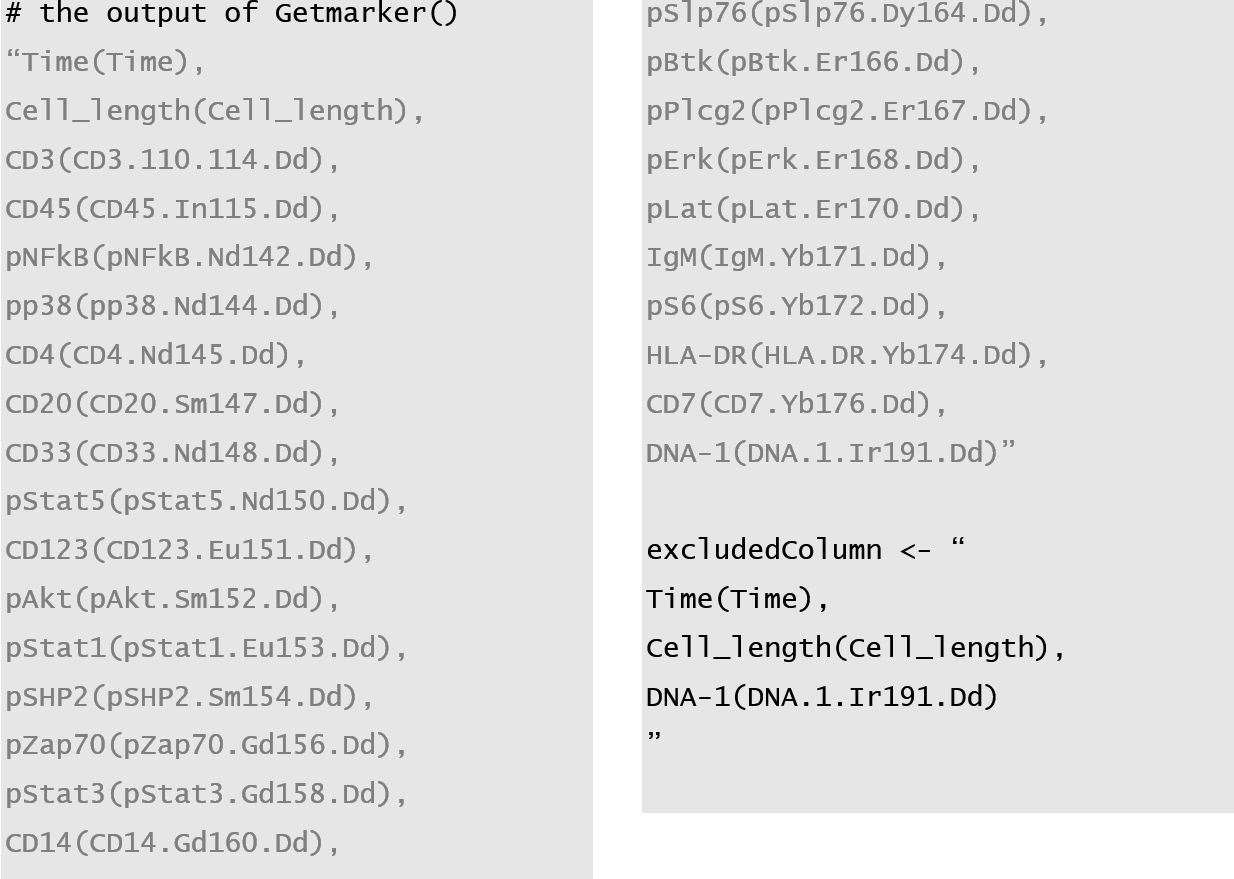
\includegraphics[width=0.7\linewidth,style="margin-left: 30px;"]{figures/Getmarker} \end{adjustwidth}

\section{Data Processing and Performance Assessment}\label{data-processing-and-performance-assessment}

The four core functions in \texttt{ANPELA}, \texttt{FC\_CSI}, \texttt{MC\_CSI}, \texttt{FC\_PTI}, \texttt{MC\_PTI}, can accomplish data processing and performance assessment in just one step, which should be used in specific condition. \texttt{FC} and \texttt{MC} denote that the raw data files are acquired from \textbf{flow cytometry (FC)} and \textbf{mass cytometry (MC)}, respectively. \texttt{CSI} and \texttt{PTI} refer to \textbf{Cell Subpopulation Identification (CSI)} and \textbf{Pseudo-time Trajectory Inference (PTI)}, respectively.

MC\_PTI sample data is a data set acquired from mass cytometry (MC), and is designed for a Pseudo-time Trajectory Inference (PTI) task. So you should use the function \texttt{MC\_PTI} to process the data and assess the performance.

The parameter \texttt{name} defines the filename of your assessment results. \texttt{cores} decides the number of CPU cores to be employed for performing parallel computing. To avoid memory explosion due to parallel computing, the default is the largest integers not greater than half of the number of CPU cores on the current host. You can also adjust your \texttt{cores} according to your specific needs, especially when handling extensive data files.

\begin{Shaded}
\begin{Highlighting}[]
\NormalTok{name }\OtherTok{\textless{}{-}} \StringTok{"MC\_PTI\_case"}
\FunctionTok{MC\_PTI}\NormalTok{(}\AttributeTok{name =}\NormalTok{ name, }\AttributeTok{datapath =}\NormalTok{ datapath, }
       \AttributeTok{index\_protein =}\NormalTok{ index\_protein, }
       \AttributeTok{pathwayhierarchy =}\NormalTok{ pathwayhierarchy, }
       \AttributeTok{cores =} \FunctionTok{floor}\NormalTok{(parallel}\SpecialCharTok{::}\FunctionTok{detectCores}\NormalTok{()}\SpecialCharTok{/}\DecValTok{2}\NormalTok{))}
\end{Highlighting}
\end{Shaded}

\textbf{Note}: \texttt{ANPELA} will run as many data processing workflows as possible, but certain methods require additional input. Due to the potentially large volume of data and workflows, which can consume significant time and memory, certain parameters are available to adjust the process. Besides the four core functions in \texttt{ANPELA}, more functions are available to realize the data processing and performance assessment in a costumed way. You can choose the function(s) and adjust the parameter values according to your specific needs, referring to the vignettes of functions in \texttt{ANPELA} \emph{R} package.

\section{Output}\label{output}

Through the above steps, you obtained the data processing and performance assessment output files for the MC\_PTI sample data, which are located in the \textbf{process\_res} and \textbf{assess\_res} folders, respectively.

\subsection{Results of Data Processing}\label{results-of-data-processing}

The \textbf{process\_res} folder stores the results of data processing. The format of data processing output files is determined by the parameter \texttt{save\_processed\_res}: (\textbf{1}) ``one\_folder'' denotes that successfully processed results will be saved as separate RData files in the ``process\_res'' folder; (\textbf{2})``one\_RData'' denotes that all processed results will be saved as one RData file in the ``process\_res'' folder {[}\emph{default =``one\_folder''}{]}.

\begin{adjustwidth}{\fltoffset}{0mm}
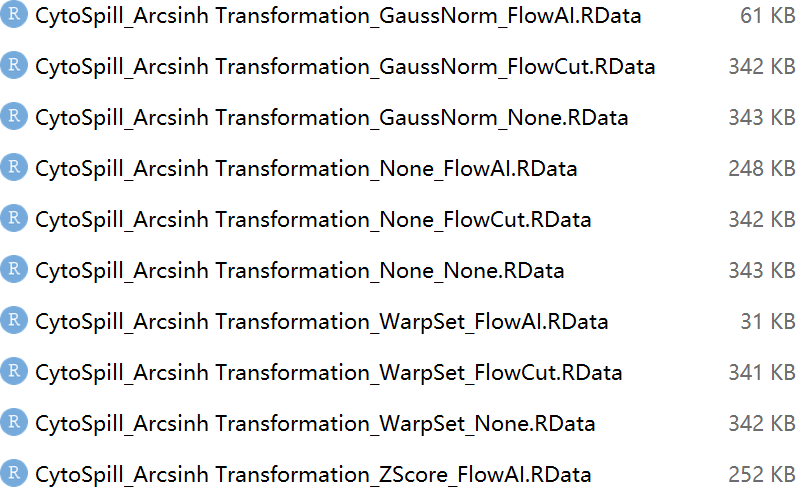
\includegraphics[width=0.7\linewidth,style="margin-left: 30px;"]{figures/process_res} \end{adjustwidth}

the folder process\_res when \texttt{save\_processed\_res = "one\_folder"}(excerpt)

\subsection{Results of Performance Assessment}\label{results-of-performance-assessment}

The \textbf{assess\_res} folder stores the results of performance assessment, which includes 3 files:

\begin{adjustwidth}{\fltoffset}{0mm}
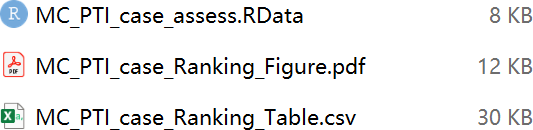
\includegraphics[width=0.5\linewidth,style="margin-left: 30px;"]{figures/assess_res_file} \end{adjustwidth}

3 files generated in the ``assess\_res'' folder

(\textbf{1}) \textbf{MC\_PTI\_case\_Ranking\_Table.csv} contains the overall ranking results of all data processing workflows, where the ``Rank'' column represents the overall ranking, and the ``Value'' column shows the scores for different assessment criteria.

\begin{adjustwidth}{\fltoffset}{0mm}
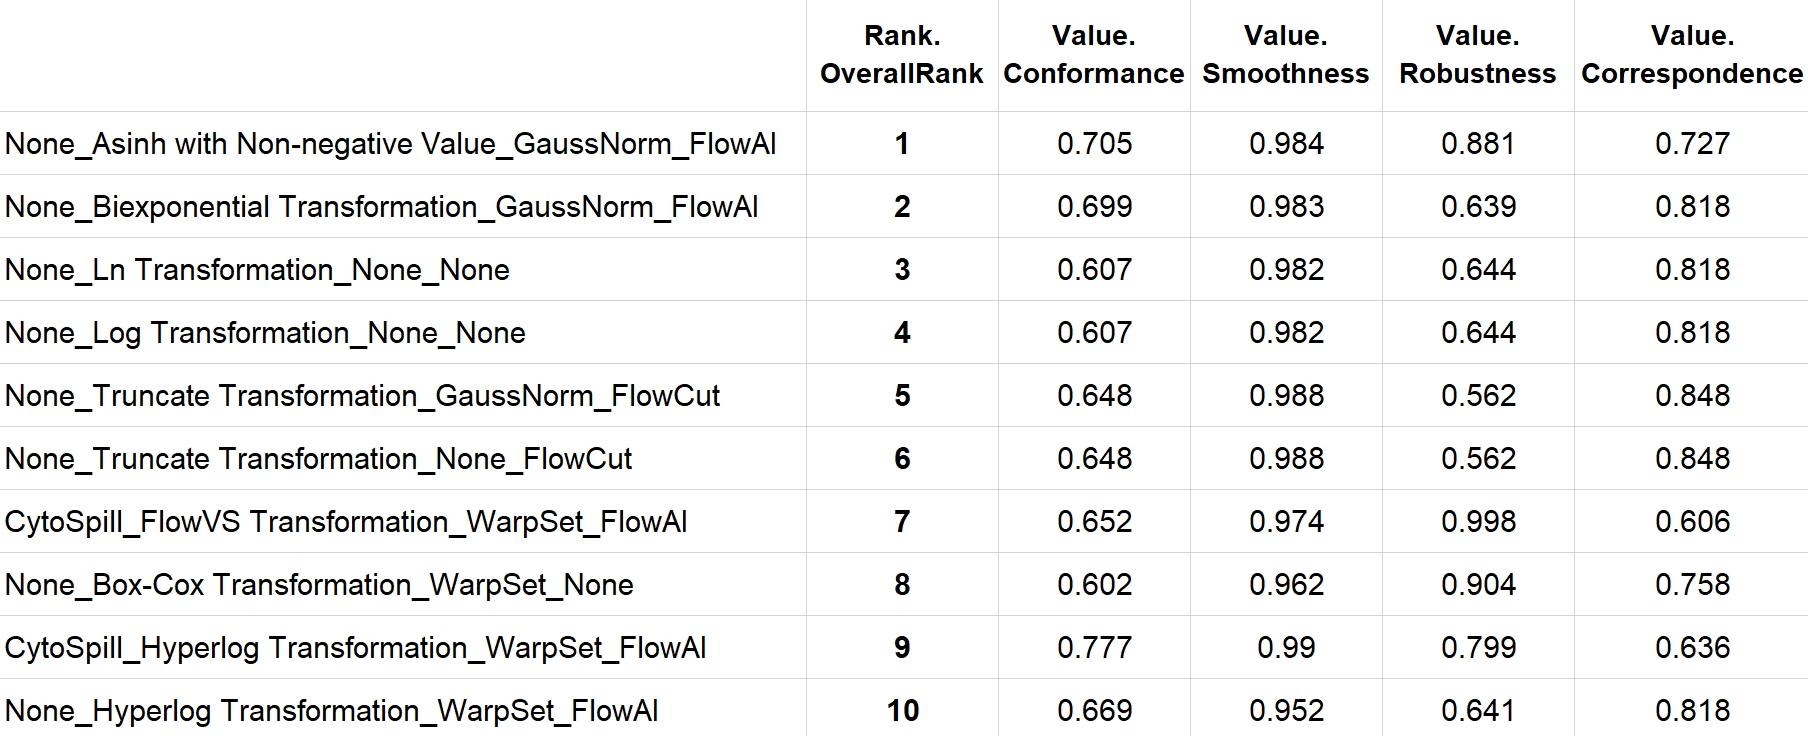
\includegraphics[width=0.95\linewidth,style="margin-left: 30px;"]{figures/assess_res_table} \end{adjustwidth}

MC\_PTI\_case\_Ranking\_Table.pdf(excerpt)

(\textbf{2}) \textbf{MC\_PTI\_case\_Ranking\_Figure.pdf} visualizes the overall ranking results to help users better understand the differences among various data processing workflows. Different colors represent different performance assessment levels: dark green indicates ``superior'', light green indicates ``good'', and red indicates ``poor''.

\begin{adjustwidth}{\fltoffset}{0mm}
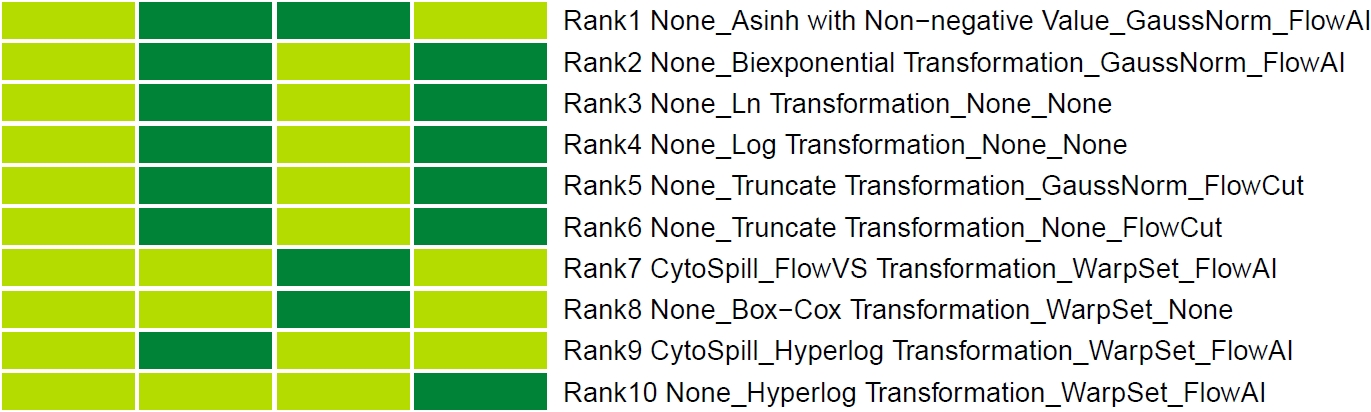
\includegraphics[width=0.9\linewidth,style="margin-left: 30px;"]{figures/assess_res_figure} \end{adjustwidth}

MC\_PTI\_case\_Ranking\_Figure.pdf(excerpt)

(\textbf{3}) \textbf{MC\_PTI\_case\_assess.RData} contains 2 tables, ``table'' and ``table2'', which provide the raw scores for different assessment criteria and performance assessment levels categorized by thresholds, respectively.

\subsection{Records}\label{records}

In addition, \textbf{log.txt} and \textbf{info\_saved.RData} files are also generated simultaneously. \textbf{log.txt} records the processing details while \textbf{info\_saved.RData} records the information related to ``metadata'' and ``index\_protein''.

\section{Reference}\label{reference}

Zhang Y, Sun HC, Lian XC, Tang J, Zhu F*. ANPELA: significantly enhanced quantification tool for cytometry-based single-cell proteomics. Advanced Science. 10(15): e2207061 (2023). doi: 10.1002/advs.202207061; PMID: 36950745


\end{document}
